\chapter{Array Fabrication and Experimental Validation}
\label{ch:array-exp}

\section{Fabrication package}
\label{sec:fabrication}
Physical fabrication specifications for every Model~B (Chapter~\ref{ch:model-b}) winning
design were generated directly from \texttt{PRIMARY\_WINNER\_PER\_M.csv}
(source: \texttt{array\_geometry\_lab/fabrication\_package/fabrication\_summary.csv},
mtime 2026-09-13 00:58, and \texttt{generate\_masks.py}, verified present): per-$M$ mask
files (positive/negative, top/bottom-mirrored SVGs), target etched hole diameter,
undercut-compensated nominal mask aperture diameter (with $\pm25\,\mu$m low/high
tolerance bounds), and blank-substrate sizing (e.g.\ $M=1$D: hexagonal, pitch
$4000\,\mu$m, target etched diameter $1250\,\mu$m, nominal mask aperture $1200\,\mu$m,
blank side $40$\,mm).

\subsection{Undercut compensation, derived in full}
\label{sec:undercut}
Wet chemical etching of the brass mask shim is isotropic: the etchant attacks sideways
under the resist edge at the same rate it etches downward, so the emerging hole is
wider than the resist opening that defined it. For a double-sided (simultaneous
two-face) etch through a shim of thickness $t$, each face etches roughly halfway
through, and the lateral undercut on each face scales with that depth:
\begin{equation}
d_{\mathrm{mask}} = d_{\mathrm{target}} - C_{\mathrm{undercut}}, \qquad
C_{\mathrm{undercut}}\in\{0.5t,\,1.0t,\,1.5t\}
\label{eq:undercut}
\end{equation}
with $t=50\,\mu$m (0.05\,mm brass shim), giving a compensation bracket of
25/50/75\,$\mu$m (source:
\texttt{Physics\_Guide/PHYSICS\_AND\_FABRICATION\_GUIDE.tex}, Equation numbered
therein as (undercut), verified read directly, mtime 2026-09-08 15:38).

\begin{warnbox}{An uncalibrated design rule, stated as such}
There is no empirical etch-rate or undercut calibration for this specific brass alloy,
thickness, etchant concentration, temperature, or agitation. The $0.5$--$1.5t$ bracket
is a standard published starting rule, not a measurement; it exists specifically
because the true value is unknown for this exact process, which is why a physical test
coupon (not merely a simulated design) is part of the fabrication plan.
\end{warnbox}

\textbf{Worked example, $M=8$D design (target etched diameter $400\,\mu$m):}
\begin{align}
d_{\mathrm{mask,nominal}} &= 400-1.0(50) = 350\,\mu\mathrm{m} & \text{(the mask actually cut)}\\
d_{\mathrm{mask,low}} &= 400-0.5(50) = 375\,\mu\mathrm{m} & \text{(least aggressive)}\\
d_{\mathrm{mask,high}} &= 400-1.5(50) = 325\,\mu\mathrm{m} & \text{(most aggressive)}
\end{align}
matching \texttt{fabrication\_summary.csv}'s own $M=8$D row exactly
(\texttt{mask\_aperture\_diameter\_um\_nominal}$=350$, \texttt{...\_low}$=375$,
\texttt{...\_high}$=325$ -- confirmed by direct read of the current file, not assumed
from the formula alone). ``Low'' and ``high'' name the assumed \emph{undercut}
magnitude, not the resulting mask diameter -- a low-undercut assumption (less lateral
etch predicted) requires a \emph{larger} mask opening to hit the same target, hence
$d_{\mathrm{mask,low}} > d_{\mathrm{mask,nominal}} > d_{\mathrm{mask,high}}$, the
inverted-looking but correct ordering visible above.

Mask registration and post-etch verification procedure are specified in full in
\texttt{Physics\_Guide/PHYSICS\_AND\_FABRICATION\_GUIDE.tex} (verified present, mtime
2026-09-08), which this paper does not reproduce beyond the undercut derivation above.

\begin{keybox}{A fix verified byte-for-byte, not merely claimed}
Because the grid-resolution defect of Section~\ref{sec:gridN} lives entirely upstream of
array geometry generation (it affects predicted \emph{blur/acuity}, not hole
\emph{positions}, which are generated deterministically from spacing parameters alone),
the fabrication package outputs were explicitly diffed before and after that fix was
applied: hole-coordinate CSVs and mask SVGs are \textbf{byte-identical} pre- and
post-fix. The fabrication geometry currently on file was never actually wrong; this was
verified directly (\texttt{diff -r}), not assumed from the fix's own scope.
\end{keybox}

\subsection{Real hole-layout diagrams, every winning design}
\label{sec:layout-diagrams}
Figures~\ref{fig:layout-gaze-weighted} and~\ref{fig:layout-worst-case} show the actual
hole positions (blue circles, to true relative scale, with the $4$\,mm pupil at
$\varphi=0$ overlaid as a dashed red circle) for every $M$ under both evaluation
models -- not schematics, the literal coordinates the fabrication masks of
Section~\ref{sec:fabrication} are cut from.

\begin{figure}[htbp]
\centering
\begin{minipage}{0.32\textwidth}\centering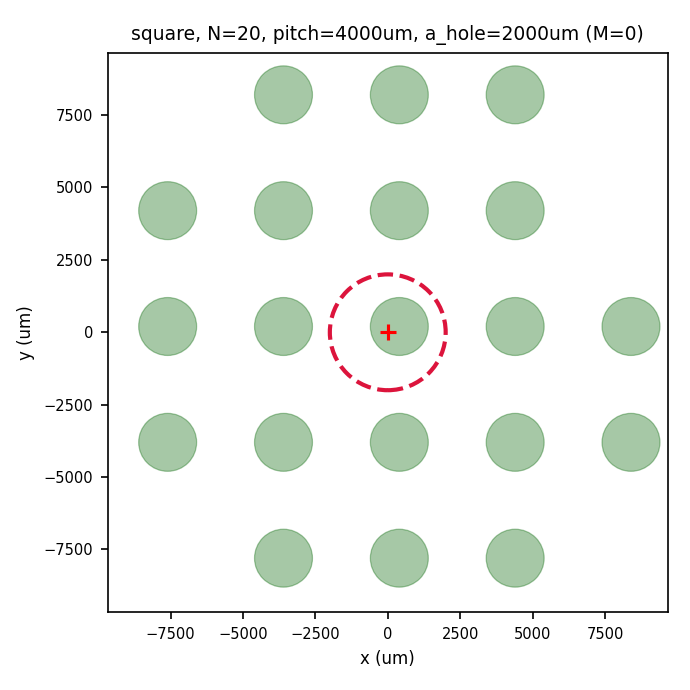
\includegraphics[width=\textwidth]{figures/GazeWeighted_M0_square_pitch4000_N20_a2000um.png}\end{minipage}
\begin{minipage}{0.32\textwidth}\centering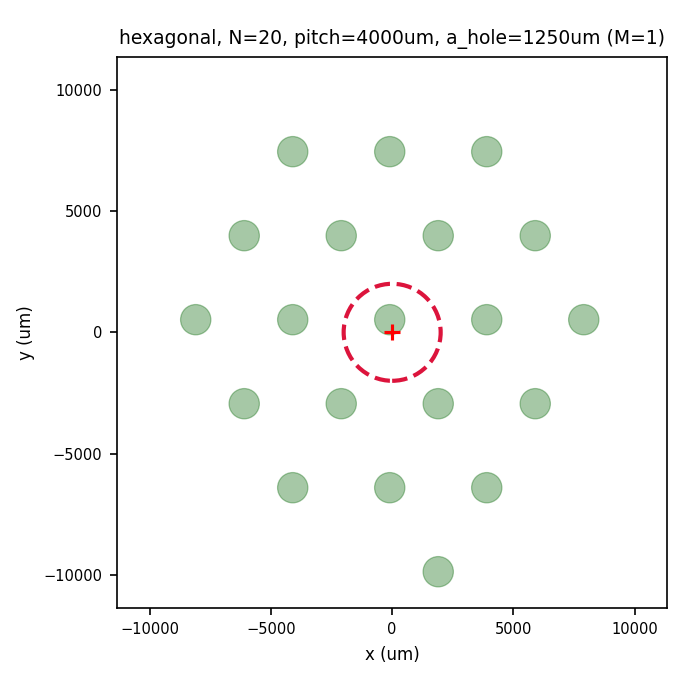
\includegraphics[width=\textwidth]{figures/GazeWeighted_M1_hexagonal_pitch4000_N20_a1250um.png}\end{minipage}
\begin{minipage}{0.32\textwidth}\centering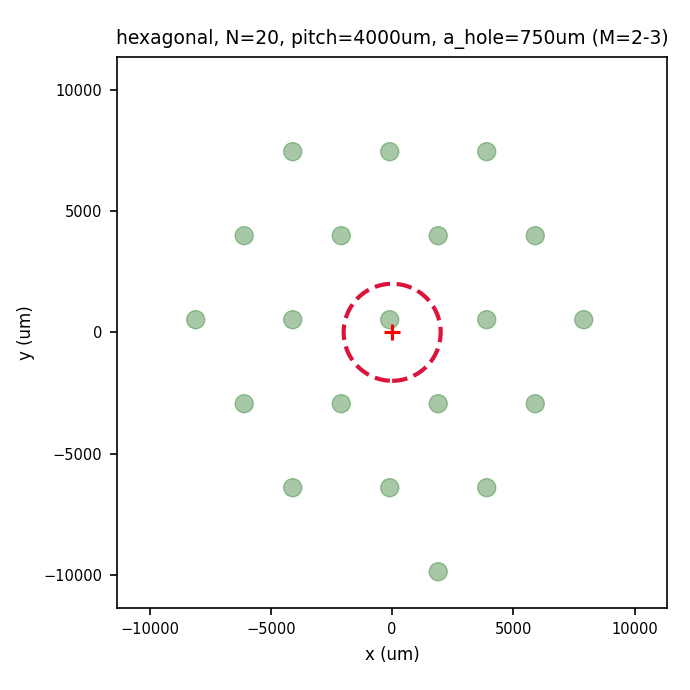
\includegraphics[width=\textwidth]{figures/GazeWeighted_M2-3_hexagonal_pitch4000_N20_a750um.png}\end{minipage}

\vspace{4pt}
\begin{minipage}{0.32\textwidth}\centering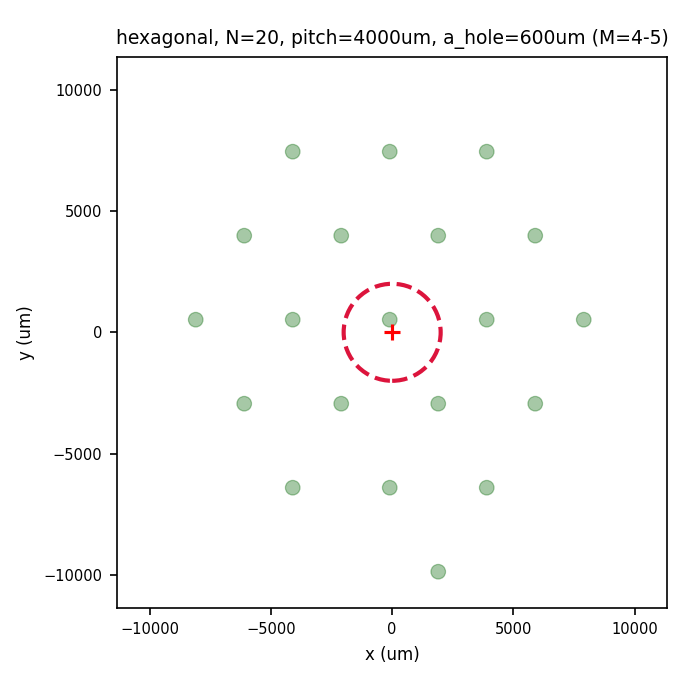
\includegraphics[width=\textwidth]{figures/GazeWeighted_M4-5_hexagonal_pitch4000_N20_a600um.png}\end{minipage}
\begin{minipage}{0.32\textwidth}\centering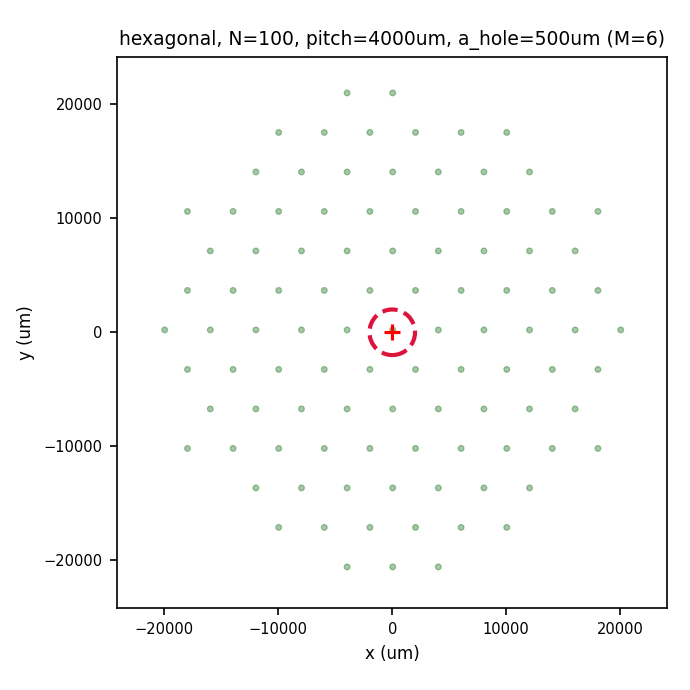
\includegraphics[width=\textwidth]{figures/GazeWeighted_M6_hexagonal_pitch4000_N100_a500um.png}\end{minipage}
\begin{minipage}{0.32\textwidth}\centering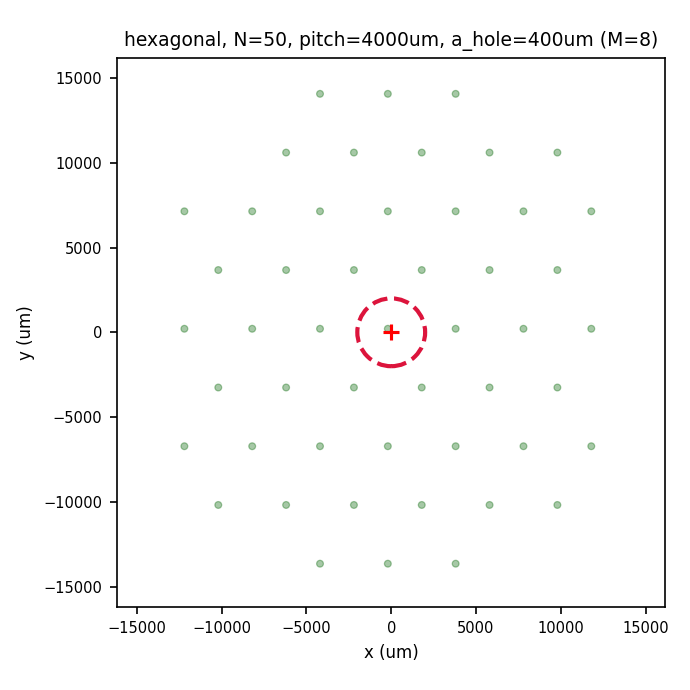
\includegraphics[width=\textwidth]{figures/GazeWeighted_M8_hexagonal_pitch4000_N50_a400um.png}\end{minipage}

\vspace{4pt}
\begin{minipage}{0.32\textwidth}\centering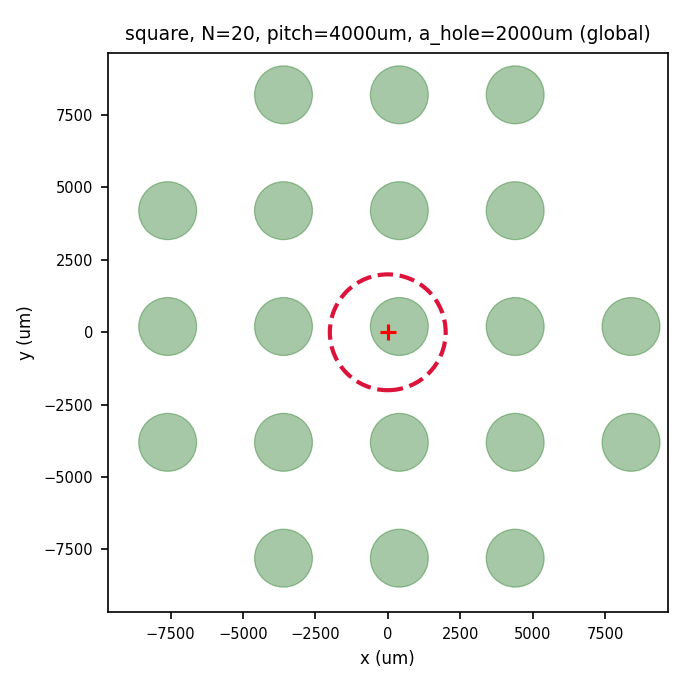
\includegraphics[width=\textwidth]{figures/GazeWeighted_Global_square_pitch4000_N20_a2000um.png}\end{minipage}
\caption{Real hole layouts, Model~B (gaze-weighted, current primary standard) winning
design per $M$ -- $M=0,1,2\text{--}3,4\text{--}5,6,8$D and the global (worst-case-across-$M$)
scope. Source:
\texttt{Array\_Design/array\_geometry\_lab/Design Visualisation/pngs\_for\_presentation/}
\texttt{GazeWeighted\_*.png}, all 7 files mtime 2026-09-17 21:32 (verified via
\texttt{stat}).}
\label{fig:layout-gaze-weighted}
\end{figure}

\begin{figure}[htbp]
\centering
\begin{minipage}{0.32\textwidth}\centering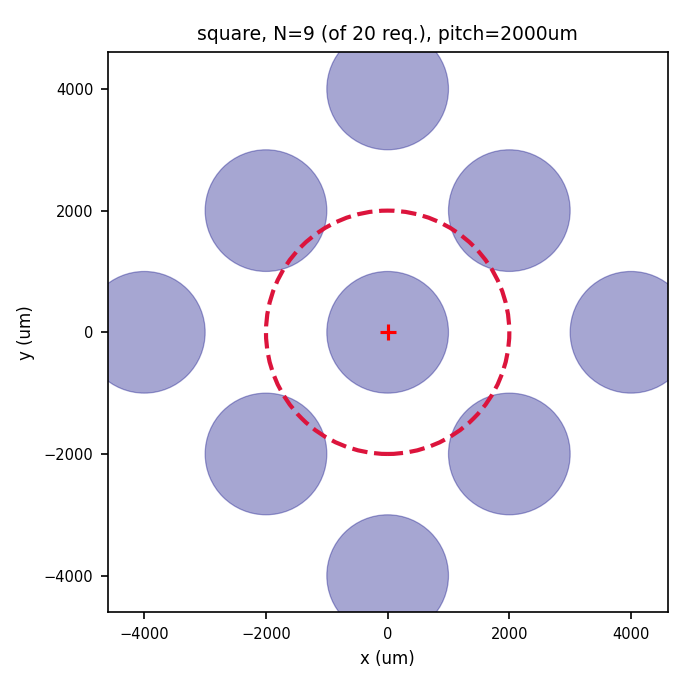
\includegraphics[width=\textwidth]{figures/WorstCase_M0_ringOffsetConcentric_rs1000_N11_a2000um.png}\end{minipage}
\begin{minipage}{0.32\textwidth}\centering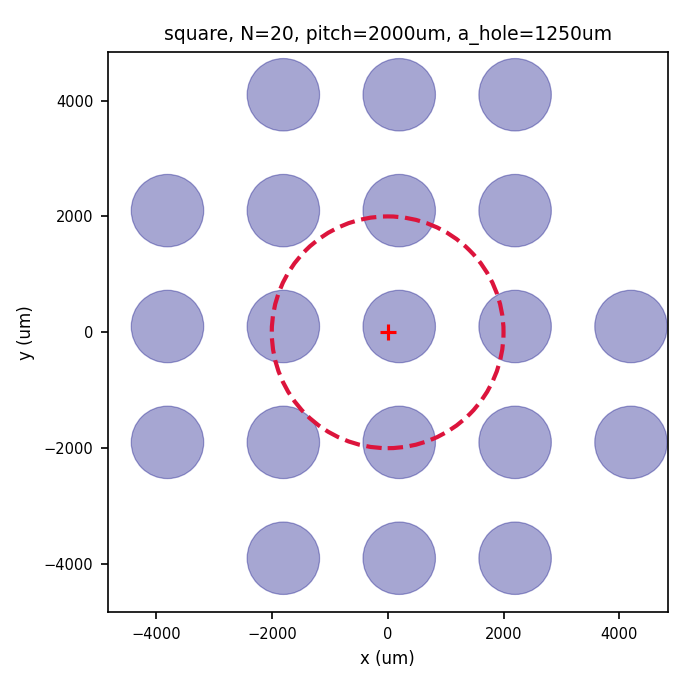
\includegraphics[width=\textwidth]{figures/WorstCase_M1_square_pitch2000_N20_a1250um.png}\end{minipage}
\begin{minipage}{0.32\textwidth}\centering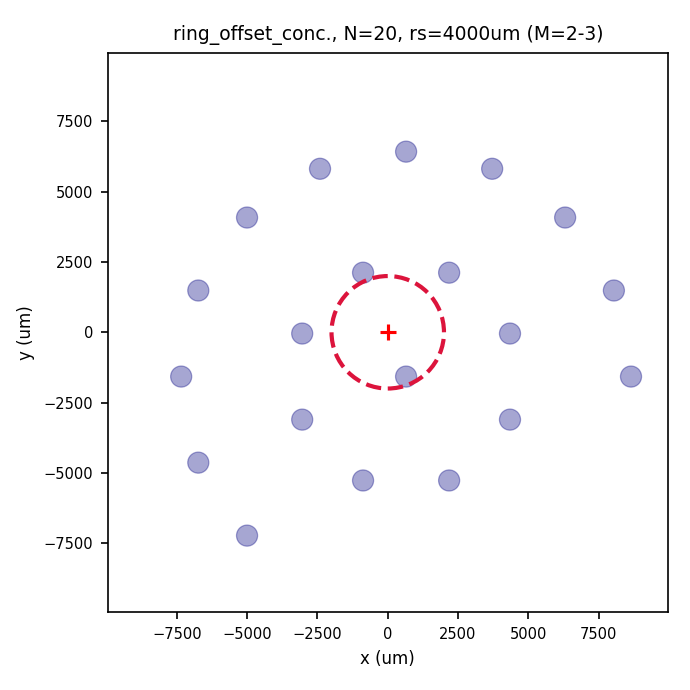
\includegraphics[width=\textwidth]{figures/WorstCase_M2-3_ringOffsetConcentric_rs4000_N20_a750um.png}\end{minipage}

\vspace{4pt}
\begin{minipage}{0.32\textwidth}\centering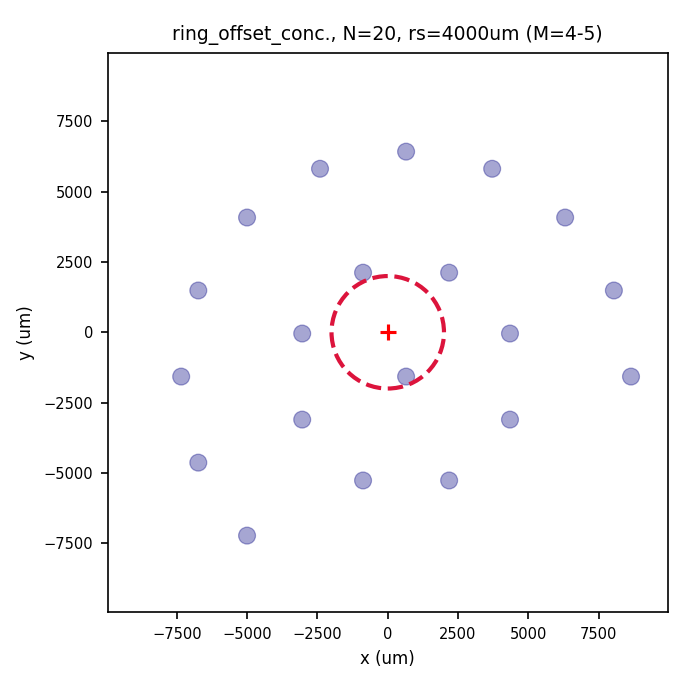
\includegraphics[width=\textwidth]{figures/WorstCase_M4-5_ringOffsetConcentric_rs4000_N20_a600um.png}\end{minipage}
\begin{minipage}{0.32\textwidth}\centering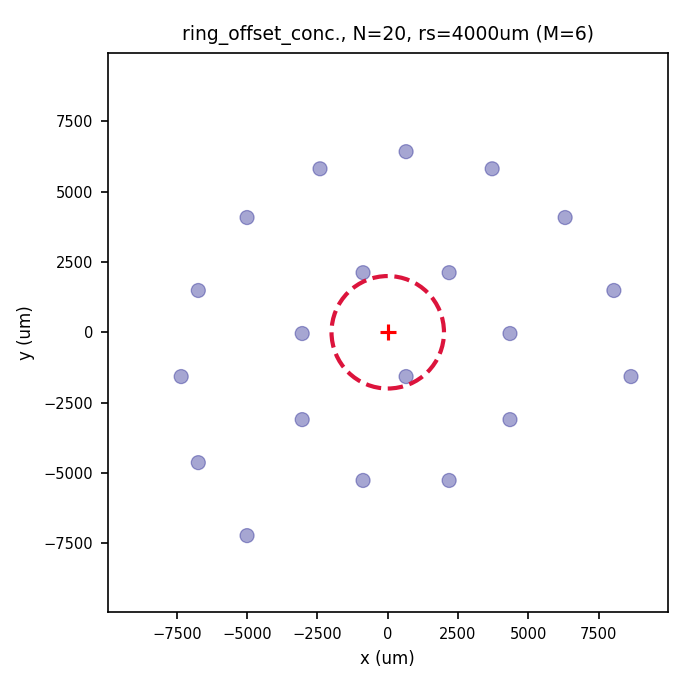
\includegraphics[width=\textwidth]{figures/WorstCase_M6_ringOffsetConcentric_rs4000_N20_a500um.png}\end{minipage}
\begin{minipage}{0.32\textwidth}\centering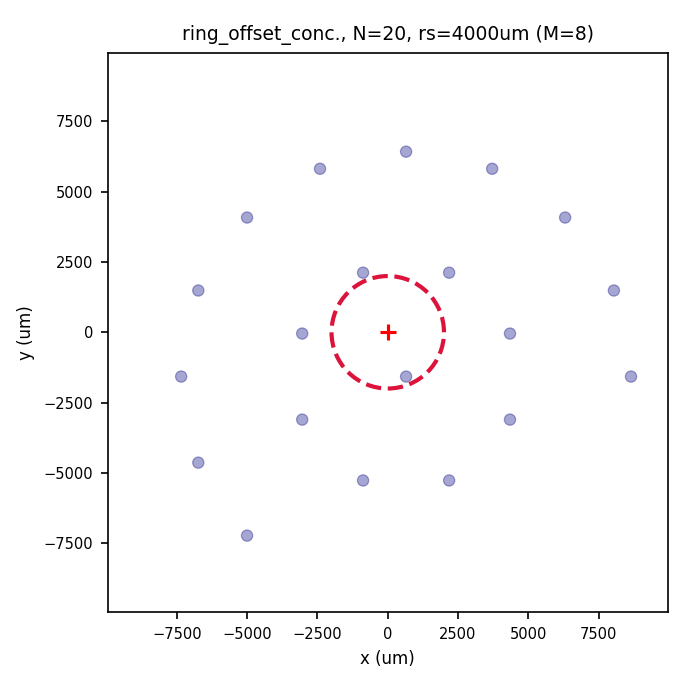
\includegraphics[width=\textwidth]{figures/WorstCase_M8_ringOffsetConcentric_rs4000_N20_a400um.png}\end{minipage}

\vspace{4pt}
\begin{minipage}{0.32\textwidth}\centering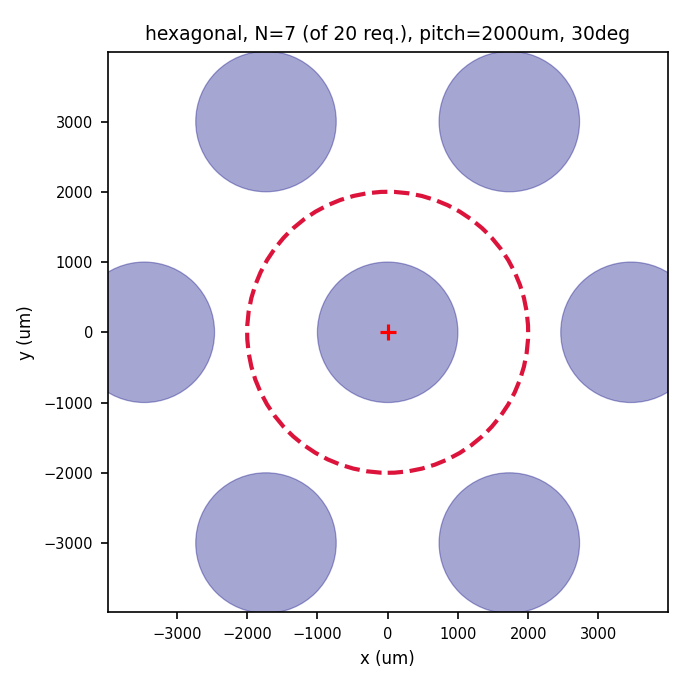
\includegraphics[width=\textwidth]{figures/WorstCase_Global_hexagonal_pitch2000_rot30_N7_a2000um.png}\end{minipage}
\caption{Real hole layouts, Model~A (single-axis worst-case gate, superseded primary
standard, Section~\ref{sec:model-a-limitation}) winning design per $M$. Note the family
mix (ring\_offset\_concentric dominates here, versus hexagonal's dominance in
Figure~\ref{fig:layout-gaze-weighted}) -- the visible consequence of the methodology
change documented in Chapter~\ref{ch:model-b}. Source: same folder as above,
\texttt{WorstCase\_*.png}, all 7 files mtime 2026-09-17 21:32.}
\label{fig:layout-worst-case}
\end{figure}

\section{Simulated retinal light-intensity distribution}
\label{sec:array-exp1}
A real ASM wave-optics simulation of the retinal intensity pattern each fabricated
design would produce, at straight-ahead gaze, was computed directly from
\texttt{stage2\_fixed/phase2\_retina.py}'s own \texttt{run\_pipeline\_point} (the same
function underlying every acuity number in this paper, Section~\ref{sec:asm}) -- not a
schematic approximation. At $\varphi=0$, every real winning design has exactly one
active hole (Table, Section~\ref{sec:model-b-results}), so the retinal image is
identical to that of a standalone single pinhole of the design's own chosen aperture.

\begin{figure}[htbp]
\centering
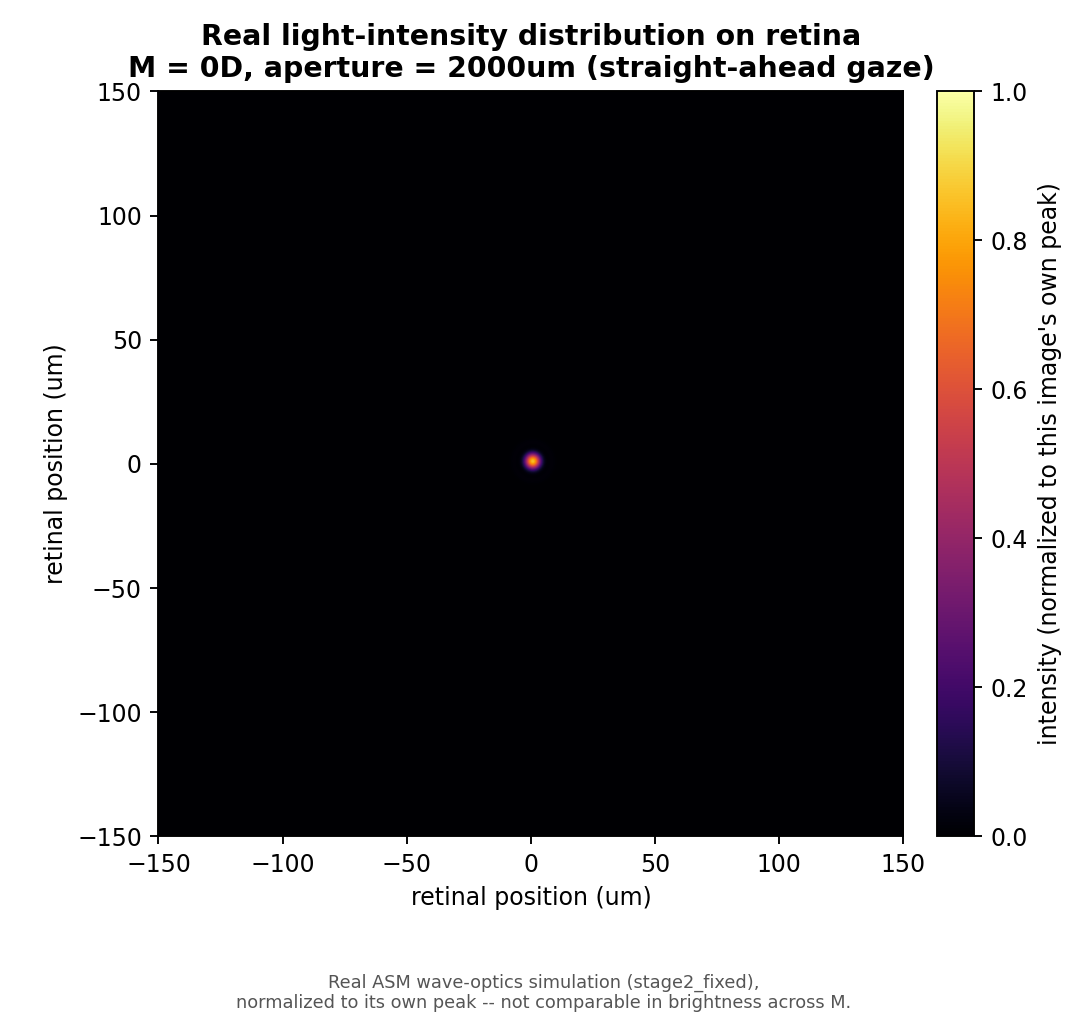
\includegraphics[width=0.30\textwidth]{figures/realistic_heatmap_M0.png}\hfill
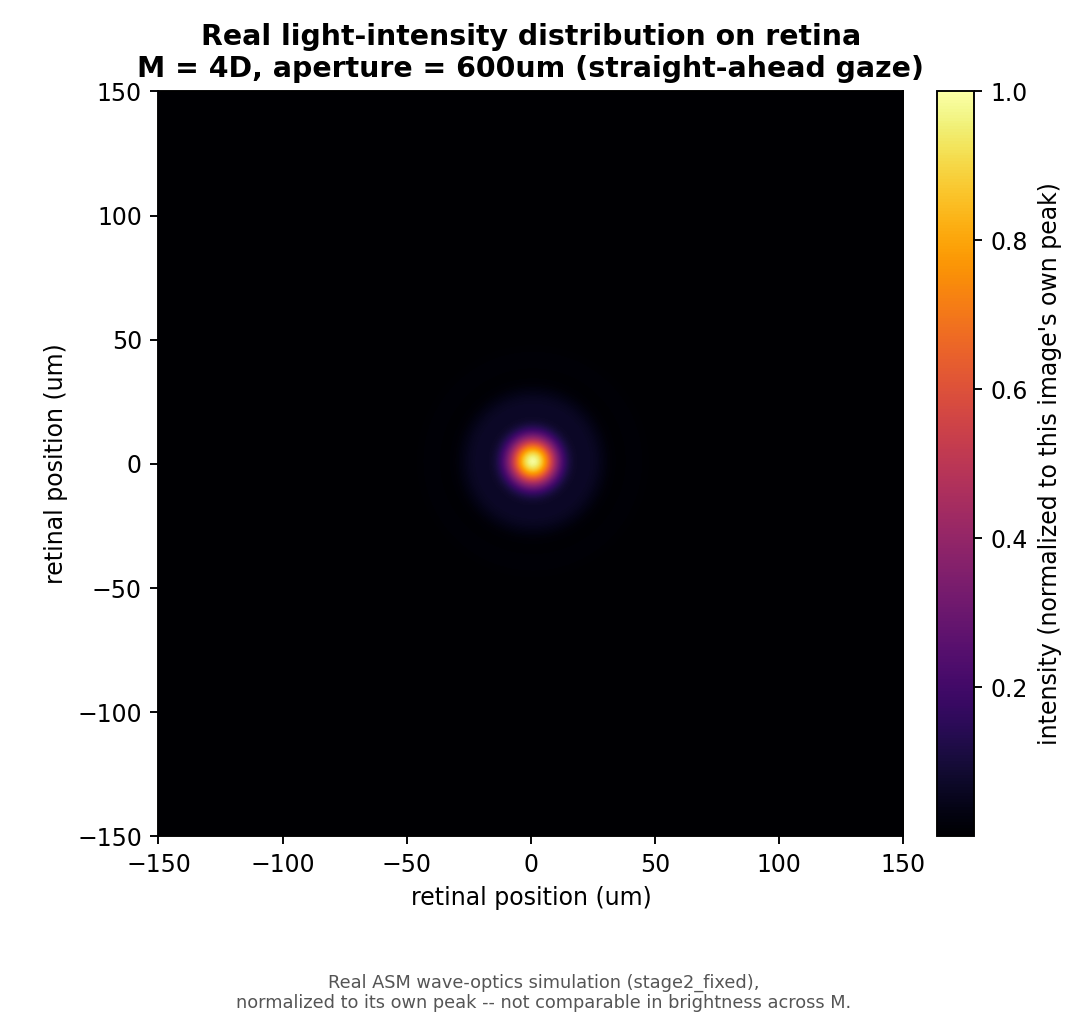
\includegraphics[width=0.30\textwidth]{figures/realistic_heatmap_M4.png}\hfill
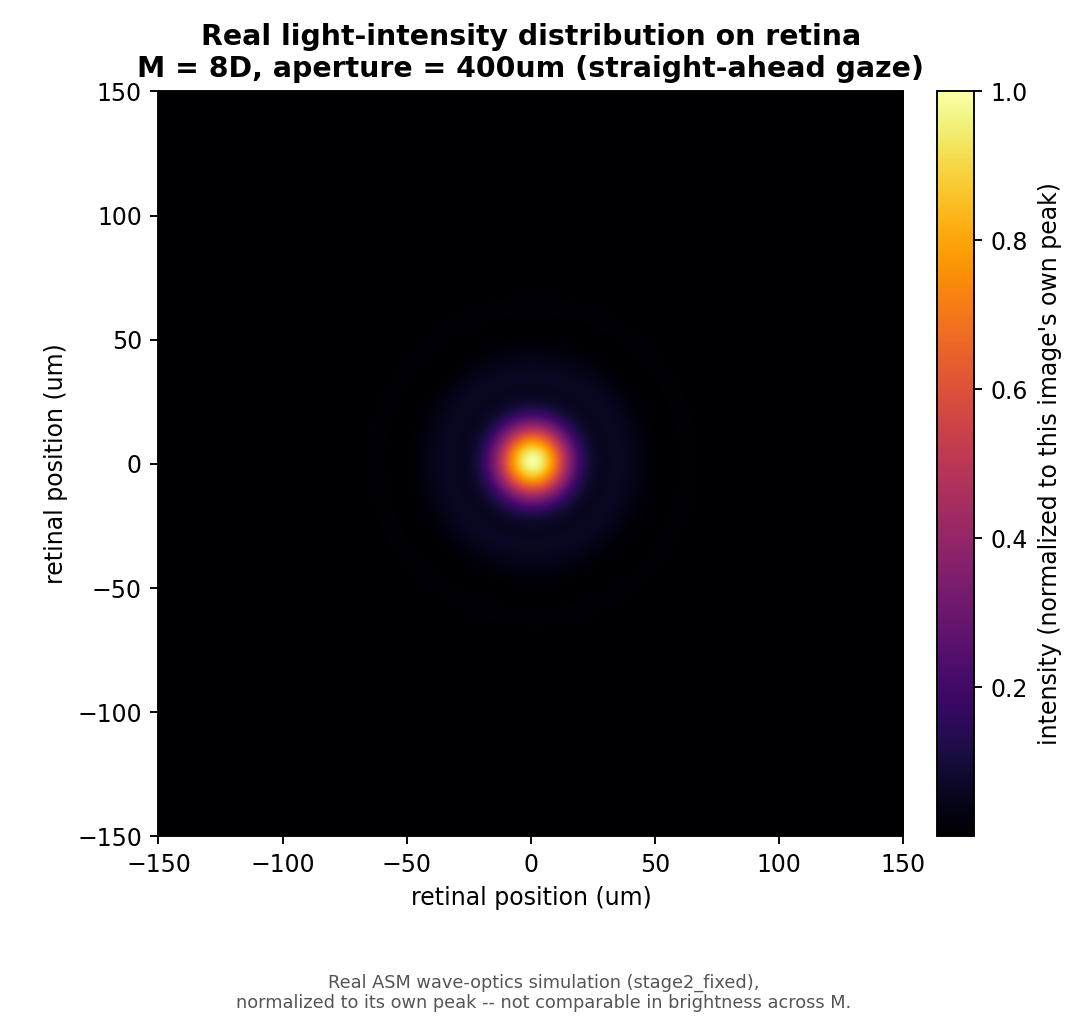
\includegraphics[width=0.30\textwidth]{figures/realistic_heatmap_M8.png}
\caption{Real, simulated retinal light-intensity distribution (straight-ahead gaze) at
$M=0,4,8$D, using each $M$'s own real \texttt{PRIMARY\_WINNER\_PER\_M} aperture (2000,
600, 400\,$\mu$m respectively). Computed directly from \texttt{stage2\_fixed}'s ASM
propagation, $N_{\mathrm{grid}}=4096$, identical parameters to the rest of this paper;
each panel normalized to its own peak intensity (absolute brightness is not
radiometrically comparable across panels without a source-power calibration this
project has not made; the blur \emph{shape} and relative \emph{size} growing from
$M=0$ to $M=8$ are real). Source: this analysis, direct call to
\texttt{stage2\_fixed.phase2\_retina.run\_pipeline\_point}; see Chapter~\ref{ch:provenance}.}
\label{fig:realistic-heatmaps}
\end{figure}

\section{A proposed physical validation rig}
\label{sec:proposed-rig}
A specific physical apparatus was designed (schematic: point source $\to$ rotating
pinhole-array insert $\to$ fixed $+20$D convex lens $\to$ a bare camera sensor (``mock
retina'') on a calibrated, Raspberry-Pi-3B+-driven linear rail) intended to measure the
real light-intensity distribution on a physical sensor as a function of simulated
myopic defocus (sensor axial displacement) and simulated gaze azimuth (array rotation).

\needsverify{As of this writing, this rig has NOT been built, and no physical
measurement data from it exists anywhere in this repository. This is stated explicitly
in this project's own animation/explainer material for the rig
(\texttt{Array\_Design/array\_geometry\_lab/proposed\_rig\_animation/}, which labels
every rendered frame ``THEORETICAL PREVIEW -- not measured sensor data''). It is
reported here as a specified, physically well-defined, but unexecuted proposal, not as
a completed experiment -- see also Section~\ref{sec:array-exp2} below and
Chapter~\ref{ch:limitations}.}

\section{Array-level clinical acuity trial}
\label{sec:array-exp2}
\begin{warnbox}{No array-level clinical trial data exists in this repository}
A search of the entire repository (every CSV for a per-subject or subject-count column,
every log file, every folder named with an experiment/clinical/trial-like pattern) found
\textbf{no} array-level, multi-subject clinical acuity trial data. What does exist is a
\emph{protocol specification} for a single-pinhole logMAR acuity measurement
(\texttt{Physics\_Guide/LOGMAR\_ACUITY\_PROTOCOL.tex}, Section~\ref{sec:logmar-protocol}),
which is explicitly designed to be extensible to a multi-subject trial but has, as far
as this repository's own files record, not yet been executed with real subjects for
either the single-aperture or the array-level case. This paper does not report, and
explicitly does not fabricate, any array-level clinical LogMAR results, deviation-vs-$M$
analysis, or subject count for this section. Any array-level clinical validation claim
made outside this document should be treated as unverified against the current
repository contents until a corresponding raw-data file is added and its provenance
recorded per Chapter~\ref{ch:provenance}.
\end{warnbox}

What this project \emph{does} have, and what Chapter~\ref{ch:model-comparison} reports
in full, is validation of the underlying single-aperture acuity model against
independently-published clinical data (Wang, 2009 \citep{wang2009}; Kim, 2017
\citep{kim2017}) -- real clinical LogMAR measurements, though not collected by this
project and not resolved per-myopia-power in the source studies. That comparison, and
its honest, unresolved statistical shortfall, is the closest this project currently has
to an array-relevant clinical acuity check, and is treated as such, not conflated with
a genuine array-specific clinical trial.
